\documentclass[11pt,a4paper]{article}
\usepackage[margin=2.5cm]{geometry}
\usepackage[T1]{fontenc}
\usepackage{lmodern}
\usepackage{amsmath,amssymb,amsthm}
\usepackage{graphicx}
\usepackage{booktabs}
\usepackage{enumitem}
\usepackage[hidelinks]{hyperref}
\usepackage{caption}
\captionsetup{font=small,labelfont=bf}
\setlist{itemsep=2pt,topsep=4pt}
\setlength{\parindent}{0pt}
\setlength{\parskip}{0.6em}
\newtheorem{proposition}{Proposition}
\newtheorem*{definition*}{Definition}
\newcommand{\tb}{\texttt{torn-bigger-13}}
\usepackage{fancyhdr}
\pagestyle{fancy}\fancyhf{}\renewcommand{\headrulewidth}{0pt}
\fancyfoot[L]{\footnotesize Written by Claude (Anthropic) for M.~Petschack}\fancyfoot[R]{\footnotesize\thepage}
\fancypagestyle{plain}{\fancyhf{}\renewcommand{\headrulewidth}{0pt}\fancyfoot[L]{\footnotesize Written by Claude (Anthropic) for M.~Petschack}\fancyfoot[R]{\footnotesize\thepage}}

\title{Learning the symmetric group: what the models learned\\[4pt]\large Interpretability and generalisation of the models of arXiv:2502.12717}
\author{Written by Claude (Anthropic), an AI model\\[2pt]\small at the request of Max Petschack, as an internal note for the co-authors of arXiv:2502.12717}
\date{28 November 2026}

\begin{document}
\maketitle

\begin{center}
\fbox{\parbox{0.92\textwidth}{\small\textbf{About this note.} This note was written by Claude, an AI model made by Anthropic; it was not written by the authors of the paper. Throughout, ``I'' refers to Claude. I designed and ran the tests on the trained checkpoints, wrote the analysis code and drew the figures. Max Petschack supplied the paper, models, code and data, ran all training on the cluster, set the questions, and corrected several of my conclusions along the way. The work up to the morning of 27 November 2026 was done by Claude Sonnet 5.5; everything after that, including this note, was done by Claude Opus 5.5 (Section~\ref{sec:timeline}). The interpretations and any errors are mine, and every number can be checked against the code and results in \texttt{Midataur/permutations-redux}.}}
\end{center}

\begin{abstract}
In this note I summarise a three-day study of the models from~\cite{paper}. The main result is an explanation of the generalisation from $S_{10}$ to $S_{25}$: each output entry depends only on a short chain of letters, and every chain that appears in a test word also appears, up to relabelling, in the training distribution. I prove the second statement with explicit constants. The elementary model generalises in the same way, and also extends somewhat past the chains it was trained on. The naive window method fails for a different reason; its chains are all covered, but its training words never contain letters far from a chain, so the model never learns to ignore them. Two windows at independent offsets are already enough to fix this. The block structure in Figure~5(b) turns out to appear in about half the runs with the same configuration, at a different place each time, and chains that cross it are no harder to follow. I suspect it is a symmetry broken by the first layers' local attention rather than anything to do with the group or the data. Finally, probes, activation patching and head ablation point to an algorithm that builds, at every letter, where a pointer leaving that letter ends up, with a reach that grows like pointer jumping.
\end{abstract}

%=====================================================================
\section{Summary and scope}

In~\cite{paper}, a transformer trained on words of transpositions in $S_{10}$ (relabelled into $S_{25}$) computes the permutation of words in $S_{25}$ with near-perfect accuracy. With adjacent transpositions and partitioned windows, a model trained on $S_{10}$ works on $S_{16}$. The paper left several things open: why this works, whether the models found a general algorithm, why the naive window method failed, and what the block substructure of Figure~5(b) means. This note covers what I found on each of these, using the paper's two trained models, about 200 other checkpoints from Max's earlier runs, and four new training runs.

In short, I found the following.
\begin{enumerate}
  \item \textbf{The block structure} (Section~\ref{sec:blocks}) is not a property of the group, the data or the task. It forms in roughly half the runs with the Figure~5(b) configuration, at different places. The first layers use it, but nothing downstream needs it.
  \item \textbf{The generalisation} (Section~\ref{sec:general}) is explained by locality and coverage. Each output entry depends only on its chain of letters, and every chain that occurs in a test word occurs often in training (Proposition~\ref{prop:coverage}). The naive window method covers every chain too; it fails because it never teaches the model to ignore distant letters.
  \item \textbf{The algorithm} (Section~\ref{sec:algorithm}) links letters through the points they share and composes chains with a reach that roughly doubles with each layer. The answer is read off the word positions in the last block.
\end{enumerate}

I have made a number of simplifications, and it is worth stating them up front.
\begin{enumerate}
  \item Each run is a single checkpoint with a single seed. Where I compare runs, the differences could partly be run-to-run noise.
  \item Accuracies are teacher-forced at one output slot at a time, unless stated otherwise. This isolates the slot being studied, but it is not quite how the model is used.
  \item Probes are linear. A quantity that a linear probe cannot read may still be present in some other form.
  \item Many tests use \emph{planted} words, built so that one slot has a chain of a chosen shape. These let me test long chains that natural words almost never contain, but they are not drawn from the test distribution.
  \item The naive-window models I tested (Section~\ref{sec:window}) are earlier runs at a smaller word length, not the paper's final elementary setup.
\end{enumerate}

%=====================================================================
\section{The pointer picture}\label{sec:pointer}

Everything below rests on a simple reformulation of the task. I use the conventions of~\cite{paper}: a word is a sequence of $N$ letters, and the output is the permutation $p=(p_1,\dots,p_n)$.

\begin{definition*}
Fix an output slot $k$. Place a pointer on point $k$ and read the word \emph{from right to left}. A letter $s_{a,b}$ (in the adjacent case, $s_{a,a+1}$) moves the pointer to $b$ if it sits on $a$, to $a$ if it sits on $b$, and leaves it alone otherwise. Then $p_k$ is where the pointer ends up.
\end{definition*}

The letters that move the pointer are the \emph{hop letters} of slot $k$, and the walk of points the pointer visits, together with the positions of its hop letters, is the \emph{chain} of slot $k$. I write $L$ for the number of hops and $s$ for the number of distinct points visited (the starting point included); in the adjacent case the \emph{width} is the length of the interval the walk covers. This picture agrees with the stored permutations of the real data in every word I checked.

The point is that $p_k$ is determined by the chain alone; every other letter only has to avoid the pointer. In a uniform test word of $S_{25}$ with $N=25$, a letter moves a given pointer with probability $48/625\approx0.077$, so a slot makes about 2 hops on average, and the longest chain in the paper's test file has 9 hops through 9 points. Training words live on 10 points, so a letter moves a pointer far more often (probability $0.18$), and the longest chains in the 8 million training words have 18 hops.

The models I use are \tb{} (the paper's general model: 5 blocks, trained for 161 epochs on a static file of 8M words) and \texttt{elem-partitioned-long-boosted-1} (the paper's elementary model, behind Figure~5(b): $n=16$, $N=120$, partitioned windows). I also use four runs that Max trained for this study with the same architecture: \texttt{g\_m10}, which uses the paper's general distribution but fresh words at every step; \texttt{g\_plant10}, in which half the words contain planted long chains (still on 10 points); an 8-block version of it; and an elementary run, \texttt{e\_base}. Finally, I use the final checkpoints of Max's earlier runs on Spartan, including the January 2025 naive-window models.

%=====================================================================
\section{The block structure of Figure 5(b)}\label{sec:blocks}

In Figure~5(b) the 120 word positions split into two blocks, positions $0$--$71$ and $72$--$119$, and the output positions form a third block. The first question is whether this comes from the data, the task, or the particular run.

It does not come from the data. The training words are position-stationary, meaning that every letter is drawn in the same way regardless of where it sits, and a per-position check of token frequencies, chain statistics and window spans finds nothing special at position 72.

To see whether it is particular to the run, I scored every elementary checkpoint on Spartan with a boundary detector. For each position $b$, the detector measures how much rows $b$ and $b+1$ of the position-cosine matrix differ away from the diagonal, as a robust $z$-score; untrained models never score above $2.5$. Figure~\ref{fig:blocks} shows the result for four runs with the configuration of Figure~5(b). Of the six fully trained runs with this configuration, three have a clear boundary (at 72, 78 and 81), one has a weak one (at 79) and two have none. An earlier run with the older architecture has the sharpest boundary of all, at 69. Where a boundary exists it lies 58--68\% of the way along the word, but its presence does not follow the length of training (63 to 341 epochs), the final accuracy, or the seed. This confirms the remark in~\cite{paper} that the structure ``was not always observed''.

\begin{figure}[t]
\centering
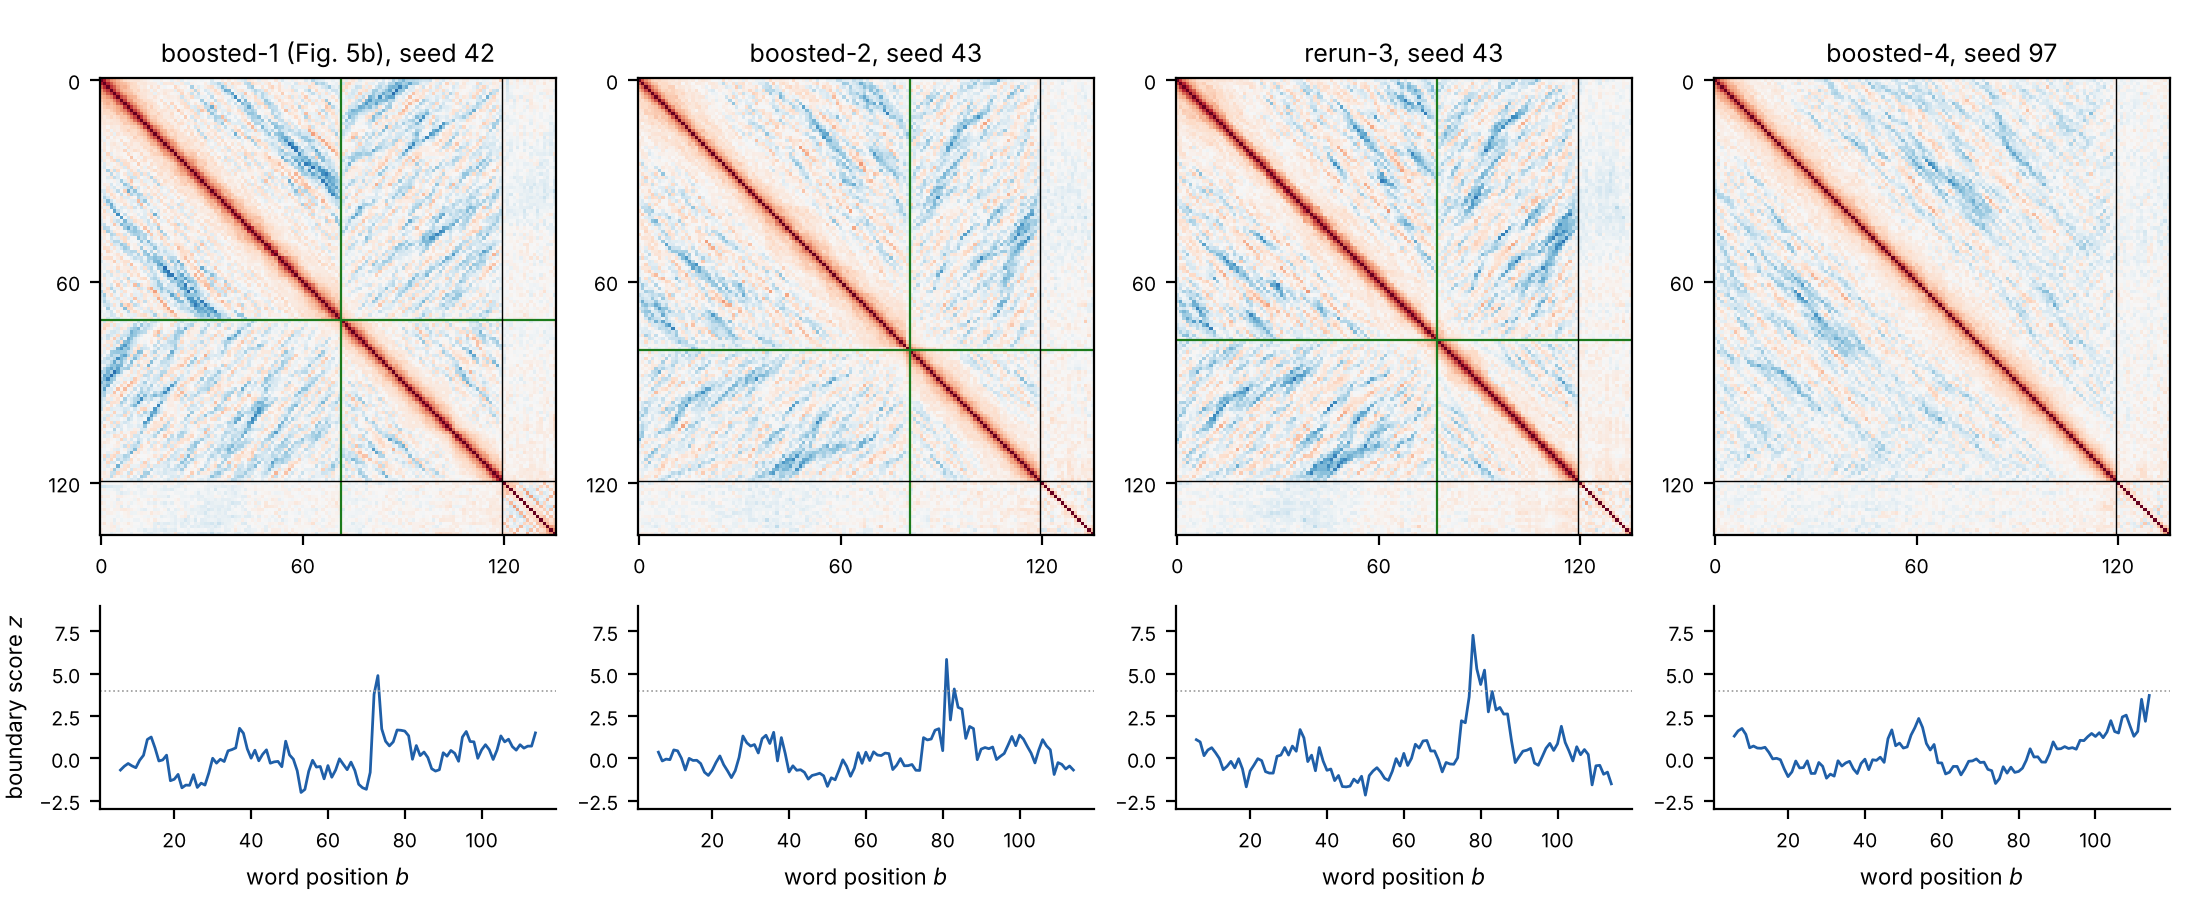
\includegraphics[width=\textwidth]{fig_blocks.png}
\caption{Cosine similarity of the position embeddings (top) and the boundary score (bottom) for four runs with the configuration of Figure~5(b) of~\cite{paper}. The first panel is that figure's model. Green lines mark detected boundaries; the black line separates word positions from output positions.}
\label{fig:blocks}
\end{figure}

The network does use the boundary, but only in its first layers. In every model with a boundary, several heads of block~1 (and some of block~2) put far less attention across it than elsewhere: between letters at most 6 positions apart, they give the boundary 4\% to 56\% of their usual weight. Models without a boundary show no such coordinated dip.

Nothing further downstream appears to need it. Chains of 24 hops placed across the boundary are followed exactly as well as chains inside one block. Swapping entries of the position-embedding table makes the model's answers follow the rearranged word in 92.6--93.6\% of the affected slots, whether or not the swap crosses the boundary. Runs without a boundary are just as accurate. I also ruled out two more specific roles: the query does not read the letters next to the boundary, and the boundary is not a single ``which half'' direction in the embeddings.

My best explanation is a form of spontaneous symmetry breaking. The first layers link each letter to nearby letters that share a point (Section~\ref{sec:algorithm}), and in a 120-letter word most candidates for that link are distractors, so these heads benefit from attention that stays local. One cheap way to help with this is to make the positions in one stretch of the word alike and unlike those in the other, so that a head can gate on ``same side''. Since the later blocks bridge the split, the loss barely depends on where it falls; each run settles wherever its details push it, and some runs never split at all. I cannot derive why the split lands 58--68\% of the way along. The right-hand part of the word, which is read first, holds the first hops of every chain, and that may make it worth separating, but this is speculation. The hypothesis predicts that in training snapshots the boundary and the heads' avoidance of it should appear together and early, and that projecting the boundary out after training should cost very little. I have tested neither.

%=====================================================================
\section{Why the generalisation happened}\label{sec:general}

The short answer has two parts. Each output entry depends only on a short chain of letters (\emph{locality}), and every chain that occurs in a test word also occurs in the training distribution, up to the symmetry (\emph{coverage}). The elementary model adds a lesson of its own: locality has to be learned, and the naive window method does not teach it.

\subsection{Locality}

To test locality, I replaced every letter of a test word that cannot touch slot $k$'s pointer with another such letter. The prediction at slot $k$ was unchanged in 98--100\% of 800 words per set, for natural words and for planted chains of up to 12 hops, whereas replacing a single hop letter changed it about 96\% of the time. The token embeddings are also close to $S_{25}$-invariant. So the trained model behaves as a function of the chain up to relabelling, which is exactly what the pointer picture says it should be.

\subsection{Coverage for general transpositions}

The two distributions to compare are the test words, in which each of the 25 letters is uniform over the 625 tokens $(a,b)\in[25]^2$, and the training words, which pick a uniformly random set $M$ of 10 of the 25 points and then draw 25 letters uniformly from the 100 tokens on $M$.

\begin{proposition}\label{prop:coverage}
Let $c$ be a labelled chain of a slot: $L$ hop letters at given positions, with a walk visiting a set $V$ of $s$ points. The ratio of its probability under the training distribution to its probability under the test distribution is
\[
R(L,s)=\frac{\binom{25-s}{10-s}}{\binom{25}{10}}\Big(\frac{625}{100}\Big)^{L}\Big(\frac{82}{100}\cdot\frac{625}{577}\Big)^{25-L}\quad (s\le 10),\qquad R(L,s)=0\quad (s\ge 11),
\]
and the same ratio holds for the total probability of each class $(L,s)$.
\end{proposition}
\begin{proof}
A hop letter must be one of the two tokens $\{(x,y),(y,x)\}$ for its step $x\to y$. Any other letter must avoid the pointer's current point $q$; the admissible tokens are those with no coordinate equal to $q$, plus the diagonal $(q,q)$, which moves nothing. That gives $24^2+1=577$ of the 625 test tokens and $9^2+1=82$ of the 100 training tokens. Since letters are independent,
\[
P_{\mathrm{test}}(c)=\Big(\tfrac{2}{625}\Big)^{L}\Big(\tfrac{577}{625}\Big)^{25-L},\qquad P_{\mathrm{train}}(c)=\Pr(V\subseteq M)\Big(\tfrac{2}{100}\Big)^{L}\Big(\tfrac{82}{100}\Big)^{25-L},
\]
where $\Pr(V\subseteq M)=\binom{25-s}{10-s}/\binom{25}{10}$, which is zero for $s>10$. Both distributions are invariant under relabelling the 25 points and under moving the hop letters to other positions, so every labelled chain in the class $(L,s)$ has the same ratio, and hence so does the class.
\end{proof}

A simulation of $10^6$ words from each distribution reproduces $R$ in every class with enough samples; for example, $(L,s)=(4,4)$ gives $2.105$ against the formula's $2.101$, and $(8,8)$ gives $12.96$ against $12.91$.

The consequences are quite strong. The only chains missing from training are those through 11 or more points, which make up $1.2\times10^{-6}$ of test slots, and the paper's test file contains none of them. Over the slots of the real test file, $R$ is never below $0.055$ (its median is $0.13$), and even the rarest chain class in the test file, $(L,s)=(8,9)$, is expected about $27{,}000$ times among the $2\times10^8$ slots of the training file. So, in the space of chains up to relabelling, generalising from $S_{10}$ to $S_{25}$ needs no extrapolation at all. Every test \emph{word} lies outside the training support, but every test \emph{slot} lies inside it. I think this is the precise form of the density intuition: the training set is dense in the test set as a set of slot chains modulo $S_{25}$, not as a set of words.

\subsection{The elementary model}\label{sec:elem}

The same picture holds for adjacent transpositions, with one difference: there is no relabelling symmetry. The chain of a slot is a walk of $\pm1$ steps, so its natural parameters are its number of hops and its width.

In the paper's test words ($n=16$, $N=120$, uniform letters), chains are moderately long but narrow: the median chain has 14 hops (at most 29) and width 5 (at most 15). In the training words, chains are longer (median 16 hops, up to 76) but never wider than 11, because a window has at most 10 points. Partitioned windows place their windows at random offsets, so every chain of width at most 11 occurs at every location, and only the 0.53\% of test slots whose chain is 12 or more wide fall outside the training data.

The model nevertheless gets 99.99\% of test slots right, wide ones included, so its rule extends past what it saw. On planted chains its accuracy falls only slowly with width beyond 11 (95.6\% at width 16 with 24 hops), and it follows chains of 100 to 118 hops (92--99\%) inside a narrow window, longer than any chain I found in a sample of its training data (78). Unlike \tb{} (Section~\ref{sec:closure}), the elementary models are also equally accurate on training, validation and fresh slots at every hop count, so they do not appear to memorise.

\subsection{Why the naive window method failed}\label{sec:window}

In the naive window method, a word of $S_{10}$ is shifted as a whole to a random place in $S_n$. Its failure is not a coverage failure. The window can sit anywhere, so every chain of width at most 10 occurs at every location, and chains in uniform test words are short; with $n=25$ and $N=20$ almost all of them have at most 5 hops. Every one of them is covered.

To find what does go wrong, I tested Max's January 2025 runs that used the naive window ($n=25$, $m=10$, $N=20$, older four-block architecture). I compared them against a run with the same $n$, $m$, $N$ and architecture in which each letter falls in one of \emph{two} windows of 5 tokens at independent offsets, and against a partitioned-window run on $S_{16}$. The results are shown in Figure~\ref{fig:window}.

Both naive-window models are 100\% right on their own distribution, but on the $S_{25}$ test file they get only 80--83\% of slots right, and only 72--78\% of slots whose chain has a \emph{single} hop. Since such short chains are certainly covered, something else must be going on. Spreading the letters of otherwise identical words over a wider range of tokens lowers accuracy steadily, from 1.00 at a range of 10 to 0.74--0.82 at the full range (Figure~\ref{fig:window}a). More directly, taking a window word and replacing 2 of its letters with letters that cannot reach anything in the window lowers in-window accuracy from 1.00 to 0.91--0.96, and replacing 8 lowers it to 0.79--0.87, even though the chains become shorter (Figure~\ref{fig:window}b). The two-window run, on the other hand, is 100\% right on the $S_{25}$ test file and in every one of these conditions, and so is the partitioned run.

\begin{figure}[t]
\centering
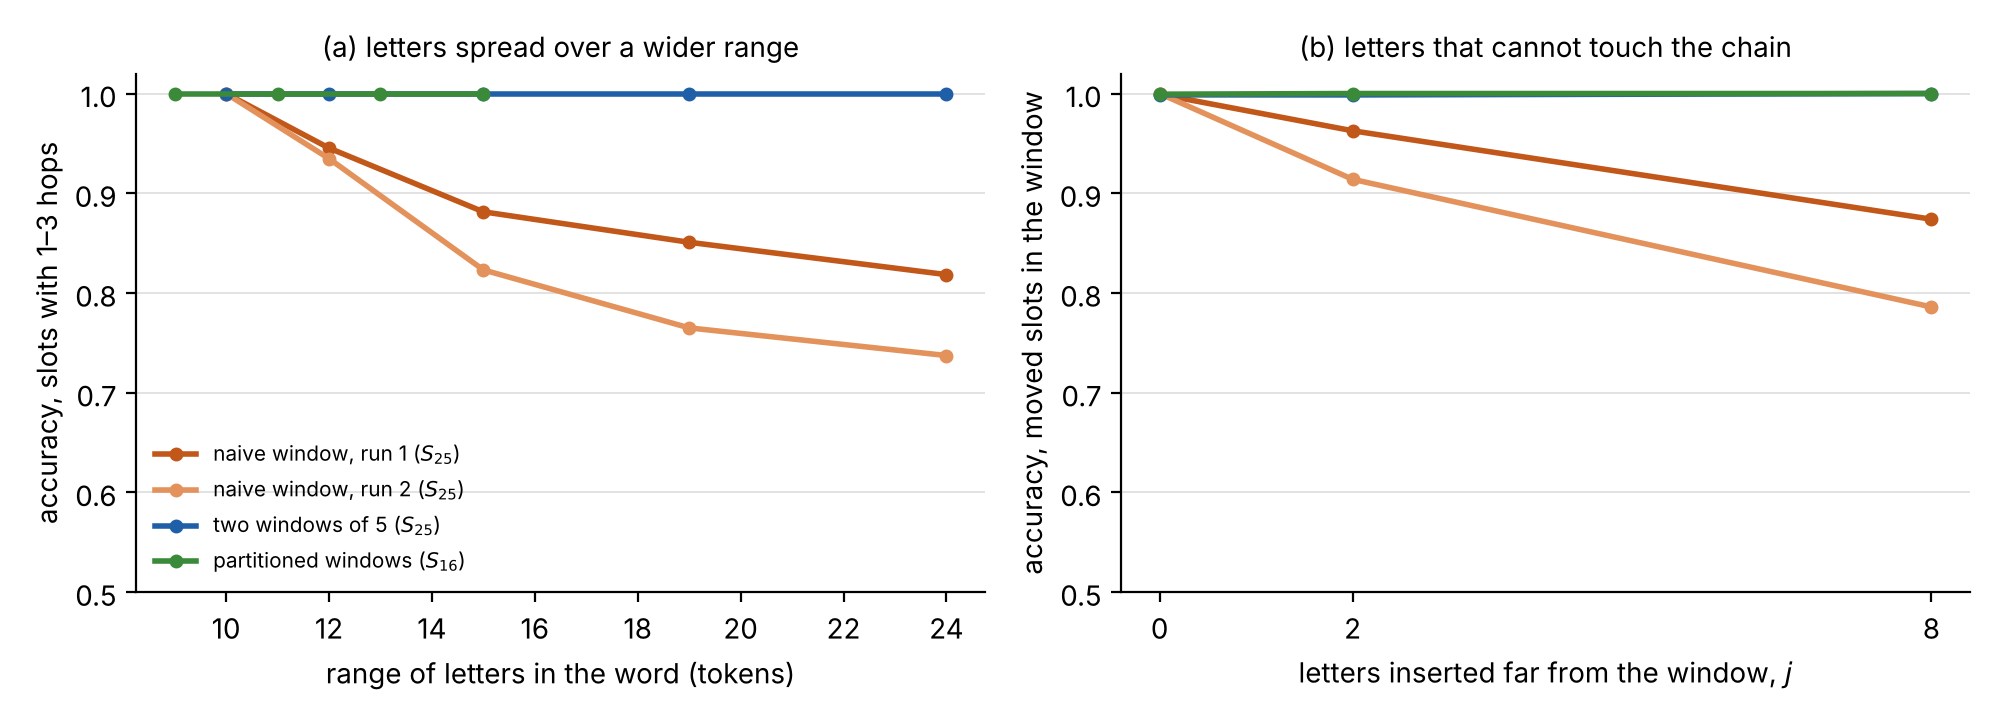
\includegraphics[width=\textwidth]{fig_window.png}
\caption{Naive against two and partitioned windows. (a) Accuracy at slots whose chain has 1--3 hops, for words whose letters are uniform over a contiguous range of tokens; a range of 10 is the naive training distribution and 24 is the full group. (b) Accuracy at the window's moved slots after inserting $j$ letters that cannot touch any chain in the window. The two-window and partitioned runs coincide at 1.00. 250 words and 6 slots per word per point.}
\label{fig:window}
\end{figure}

The explanation, I think, is that locality is not built into the architecture. Attention can look anywhere, so the model has to learn to ignore irrelevant letters, and it only learns to ignore the kinds of irrelevant letters it has seen. For general transpositions this comes for free: after relabelling into $S_{25}$, every point off the chain is equivalent to every other, and training words already contain letters on such points. For adjacent transpositions distance matters. In a naive-window word every letter lies within 10 points of every chain, so the model never meets a letter 15 points away and never learns that such a letter is harmless. Two windows at independent offsets, or partitioned windows, put letters at all distances from every chain, and that is what teaches the model to ignore them. The paper's intuition that the naive model ``learns the smaller group'' fits this picture well: it learns a function of the whole word that agrees with the group only on words that fit inside one window.

For the density argument this adds a second condition to coverage. The training distribution has to cover the chains, and also the configurations of irrelevant letters around them that the model must learn to ignore. For general transpositions the symmetry takes care of the second condition; for adjacent ones the windows have to be split for it to hold.\footnote{An earlier two-window run (\texttt{elem-wacky-1}, January 2025, before a fix to the window code) did not train, getting only 60\% of moved slots right on its own distribution.}

\subsection{Coverage is necessary but not sufficient}\label{sec:closure}

Containment in the training distribution does not guarantee that a model generalises to a given chain; frequency and the training procedure decide where the edge falls (Figure~\ref{fig:memo}). The clearest example is that \tb{} has memorised its long training chains. It is right on 100\% of its own training slots with 12 to 17 hops, but on fresh slots with the same hop counts its accuracy is noticeably lower:

\begin{center}
\small
\begin{tabular}{lcccccc}
\toprule
hops & 12 & 13 & 14 & 15 & 16 & 17\\
\midrule
fresh slots, accuracy & 0.999 & 0.989 & 0.976 & 0.943 & 0.868 & 0.72\\
training slots available & 1500 & 1500 & 1468 & 270 & 34 & 2\\
\bottomrule
\end{tabular}
\end{center}

The difference is significant at every hop count from 13 to 16, and the decline starts where the training file still holds about a thousand examples per hop count. The wandb history agrees: from about epoch 80 the training loss falls to $4\times10^{-9}$ while the validation loss stays near $10^{-5}$. Since the test file never needs more than 9 hops, none of this affects the paper's result.

Two of the new runs show that this edge is not fixed. The fresh-data run \texttt{g\_m10}, with the same distribution and about 25 times as many examples, still gets 0.93--0.95 on planted chains of 20--22 hops through 10 points, beyond any chain it saw. With planted long chains in the data (\texttt{g\_plant10}), the same five-block architecture is perfect up to 24 hops and 25 points. So the general model's limit is a property of the rule it learned, not of the architecture.

\begin{figure}[t]
\centering
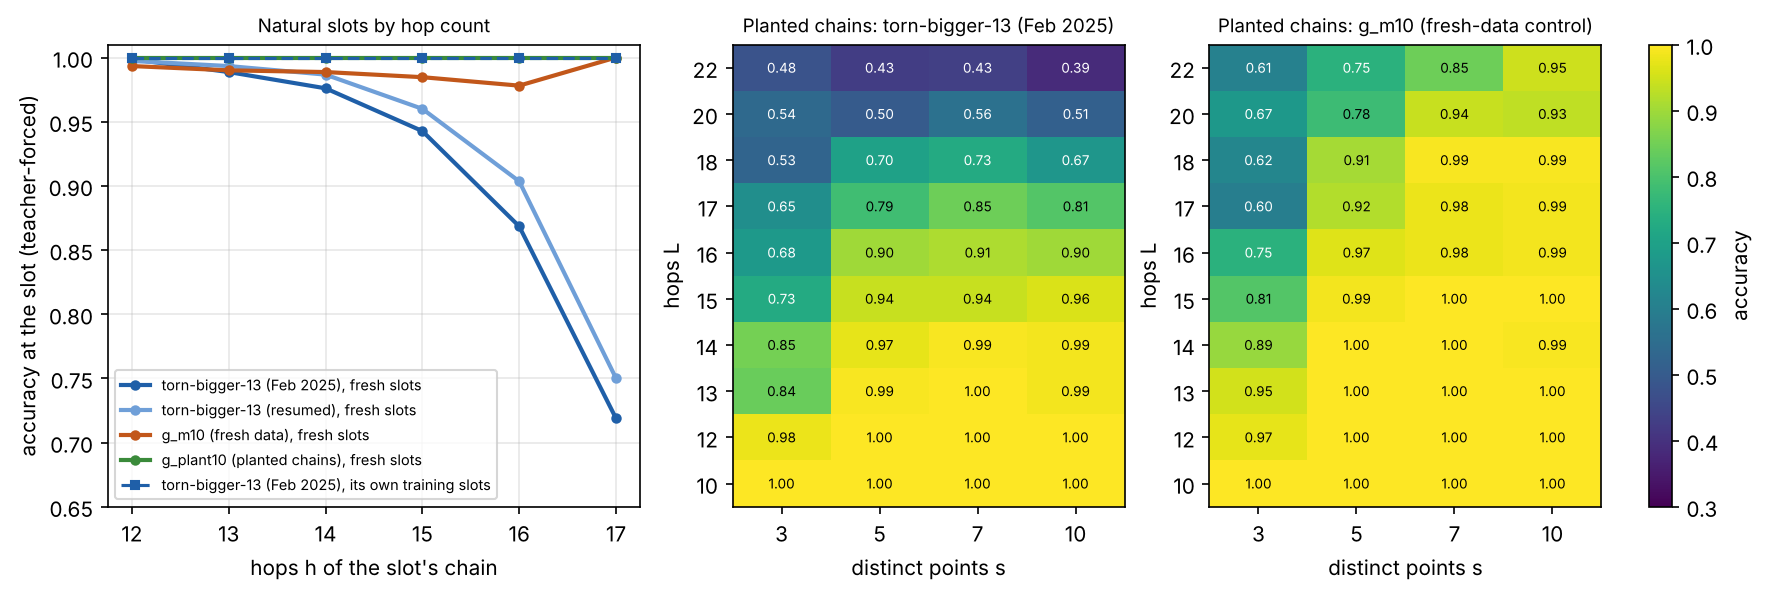
\includegraphics[width=\textwidth]{fig_memorisation.png}
\caption{Left: accuracy on natural slots by hop count, for fresh slots of several models and for \tb{}'s own training slots (top line). Middle and right: planted chains by hops $L$ and distinct points $s$, for \tb{} and the fresh-data run.}
\label{fig:memo}
\end{figure}

%=====================================================================
\section{What algorithm the models learned}\label{sec:algorithm}

To look inside the models I used four tools: linear probes~\cite{probes} on the residual stream, at both the query (output) positions and the word positions; activation patching~\cite{rome} between words that differ in one hop letter; attention patterns on planted chains, with a control on natural words; and zero- and mean-ablation of single heads and groups of heads. Most of what follows is about \tb{} and the elementary model.

The obvious guess is that the query position traces the chain one hop per layer. This turns out to be wrong. At the position that predicts $p_k$, a probe can recover where the pointer is after the first 1--4 hops, but for $L=8$ or $12$, where the model is 100\% correct, it never recovers the later hops (at most 13\%, against a chance level of 4\%).

Instead, the work happens at the word positions. For a letter, define its \emph{continuation} to be where a pointer leaving that letter ends up after the remaining letters. A probe at the word positions can decode the continuation of a letter with $h$ hops still to go, but only from a certain layer onwards:

\begin{center}
\small
\begin{tabular}{lccccc}
\toprule
layer & 1 & 2 & 3 & 4 & 5\\
\midrule
hops ahead first decodable, general model & 1 & 1 & 4 & 8 & $\ge 13$\\
hops ahead first decodable, elementary model & 1 & 2 & 4 & 8 & 12\\
\bottomrule
\end{tabular}
\end{center}

This doubling is the signature of pointer jumping~\cite{hillis}, in which each layer joins a letter's continuation to the continuation of the letter it points to. In the elementary model the attention offsets double as well: heads attend to hop letters $\pm1$ hops away in blocks 1--2, $\pm2$ and $\pm4$ in block 3, and $\pm6$ to $\pm12$ in block 4.

Activation patching shows where the answer is read from. If I corrupt a middle or last hop letter and then restore the clean activations at all word positions after block~4, the clean answer comes back in every word, even though the query position's own state was computed from the corrupted word. Corrupting the first hop can only be repaired this way up to block~3, because by then the query position has already taken in the first hops itself. Patching only the letters read \emph{before} the corrupted one repairs it, while patching those read after it does not, so information flows in the direction that continuations are built.

The heads that link letters do so by content. Heads in blocks 1--3 attend to the next or previous letter of the chain with 3--4 times (general model) and 13--40 times (elementary model) the weight they give a non-chain letter at the same distance. In \tb{}, four such heads are redundant with one another: each costs at most 3 points when zeroed on its own, but zeroing all four drops accuracy at 8 hops to 12\%.

Putting this together, the algorithm I propose has three steps.
\begin{enumerate}
  \item The first blocks link each hop letter to its neighbours on the chain, through the points they share.
  \item Successive blocks compose continuations, roughly doubling their reach each time.
  \item The query position takes in the chain's first hops by block~3, and in the last block reads the answer from the continuation stored at the word positions.
\end{enumerate}
This predicts a limit in the number of hops, not in the number of points, at about the reach of the last layer, which is what I see for \tb{}: on fresh chains it is reliable to about 13 hops whatever the number of points, and its longer training chains are memorised separately. Two parts are not pinned down. In the general model the attention offsets show the doubling only weakly, and the elementary model follows 118 hops with a probed reach of about 12, so it must compose long chains in a way a linear probe does not see. The planted model \texttt{g\_plant10} shows neither the staircase nor any hop limit, and I have not found its algorithm.

A finer test supports the content-based linking. Holding $L$ and $s$ fixed and varying only the shape of the walk (Figure~\ref{fig:shape}), cycles ($a\,b\,c\,d\,e\,a\ldots$) are easy for every model, but walks that keep returning to the point they just left ($a\,b\,a\,b\ldots$) are hard. At 16 hops through 5 points, \tb{} falls from 0.96 to 0.68 and \texttt{g\_m10} from 0.99 to 0.86; at 18 hops, they fall from 0.75 to 0.46 and from 1.00 to 0.70. This is what content-based linking would predict, since in a back-and-forth stretch every hop letter is the same pair $\{a,b\}$ and content cannot tell the next link from any other. It also means that the fresh-data run's apparent weakness on chains through few points is really a weakness on back-and-forth chains. The planted model is perfect on all of them.

\begin{figure}[t]
\centering
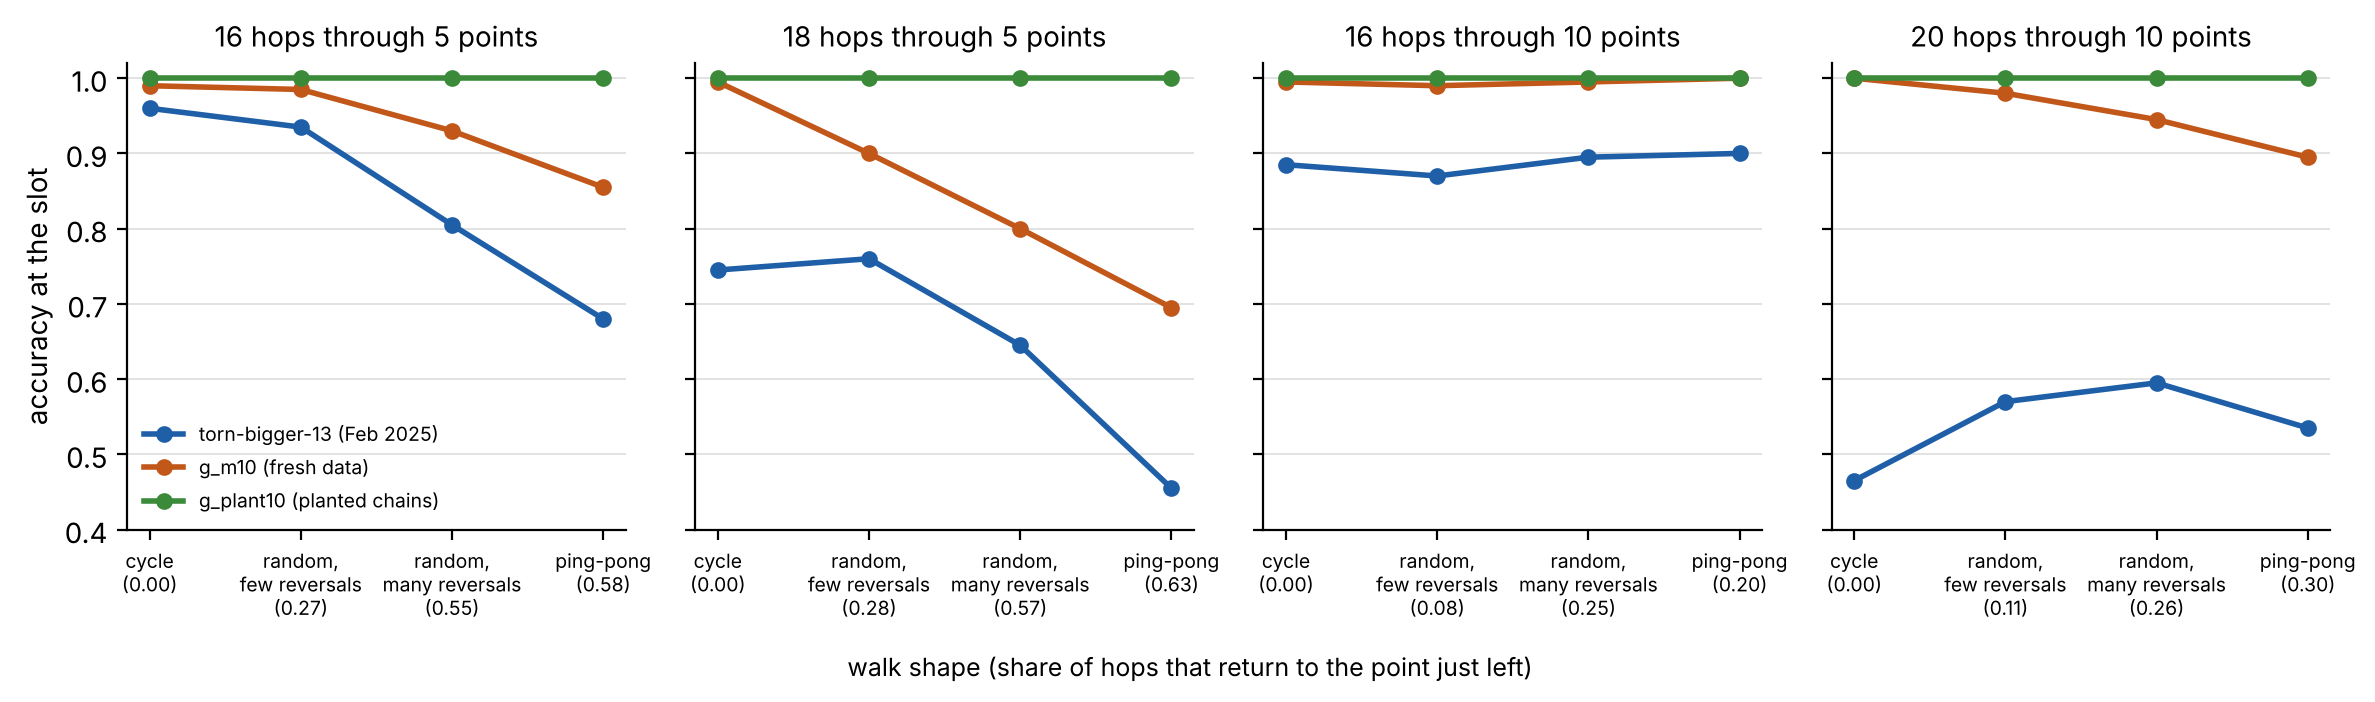
\includegraphics[width=\textwidth]{fig_pattern_families.png}
\caption{Accuracy by the shape of the walk at fixed hops and points (200 planted words per point). In brackets: the share of hops that return to the point just left.}
\label{fig:shape}
\end{figure}

%=====================================================================
\section{Conclusion and open questions}\label{sec:open}

In this note I have argued that the paper's generalisation comes down to two facts: the trained models are local, depending only on the chain that moves each output entry, and every chain in the test distribution is well covered by the training distribution once the symmetry is taken into account. The second fact can be proved outright for general transpositions. For adjacent transpositions, the naive window method covers every chain but fails to teach locality, which explains why splitting the window was necessary. The block structure of Figure~5(b) appears to be a by-product of training rather than a feature of the problem.

The study has several natural extensions, and some open questions remain.
\begin{enumerate}
  \item \textbf{Was \tb{}'s rule ever longer?} A faithful rerun with per-epoch snapshots would show whether the hop limit was there from the start, or whether it was overtaken by memorisation once the training loss reached $10^{-9}$. The run is prepared but has not yet been run.
  \item \textbf{Data or recipe?} It is unclear whether a larger static file would move the general model's edge with everything else as in the paper. The fresh-data run differs from the original in several respects at once, so it cannot answer this on its own.
  \item \textbf{How are 118 hops composed?} The elementary model follows chains ten times longer than its probed reach. Head-level patching at long chains, and a test of whether it exploits the narrowness of the walk, would be the next step.
  \item \textbf{What does the planted model do?} It shows no staircase, no hop limit and no cost for back-and-forth walks, and I do not yet understand how.
  \item \textbf{Does the block hypothesis hold?} Training snapshots of a run that forms a boundary, removing the boundary after training, and words of other lengths would all test it.
  \item \textbf{Is there a theory of closure?} Coverage is now a theorem, but what a training procedure makes of it is only measured. A description of which chains a model extends to, for instance in terms of frequent short segments composed by the layers, would complete the density argument.
\end{enumerate}

%=====================================================================
\section{Timeline and division of work}\label{sec:timeline}

The study ran from 25 to 28 November 2026. Max (M) set the questions, supplied the models, code and data, ran all training on the cluster, and corrected several of my conclusions. I (C) designed and ran the tests on the checkpoints, wrote the analysis code, and wrote the reports and this note.

The work was done by two Claude models. Up to report version~9 (27 November, 08:20 AEDT) it was done by Claude Sonnet 5.5; from the memorisation test (27 November, 09:16) onwards it was done by Claude Opus 5.5. The switch is visible in the model named in the repository's commit records. At Max's request, Claude Opus 5.5 then re-examined the conclusions of the earlier work, and several of them were revised in report version~10.

\begin{center}
\small
\begin{tabular}{p{2.2cm}p{10.0cm}l}
\toprule
date & work & by\\
\midrule
2024--25 & The paper, its models, data generator and training runs; about 200 further checkpoints. & M\\
25 Nov 2026 & Repository with the two paper models; the questions (density argument, Figure~5(b)). & M\\
25 Nov & Baseline, planted chains, the pointer picture, layer-wise probes, interventions, position-embedding ablation. & C (Sonnet)\\
25 Nov & Confirmed the model behind Figure 5(b). & M\\
26 Nov & Probes and patching at the word positions, attention and ablation, the elementary model beyond its longest chains; design of a four-arm training experiment. & C (Sonnet)\\
26 Nov & Ran the four-arm experiment on the cluster. & M\\
26--27 Nov & Analysis of the four new models (report version 8). & C (Sonnet)\\
27 Nov & Correction: distinct words against words presented (report version 9, 08:20). & M, C (Sonnet)\\
\midrule
\multicolumn{3}{c}{\textit{27 Nov, between 08:20 and 09:16: switch from Claude Sonnet 5.5 to Claude Opus 5.5}}\\
\midrule
27 Nov & Memorisation test of \tb{} (09:16). & C (Opus)\\
27 Nov & Corrections: experiments should change one thing at a time; the original used bf16. & M\\
27 Nov & Prepared a faithful rerun of \tb{} with snapshots (not yet run). & C (Opus)\\
27 Nov & Exported the wandb histories, made the wandb project public, uploaded all checkpoints. & M\\
27 Nov & Survey of all checkpoints: block boundaries across runs, which checkpoint is which, hops against points, elementary models do not memorise. & C (Opus)\\
28 Nov & Re-examination of the Sonnet-era conclusions (report version 10, at M's request). & C (Opus)\\
28 Nov & The algorithm and the density notion (at M's request); block hypothesis; coverage proof; walk-shape test; naive-window test; this note. & C (Opus)\\
\bottomrule
\end{tabular}
\end{center}

All code, results and the full reports are in the repository \texttt{Midataur/permutations-redux}, in the folder \texttt{claude-analysis/}.

\begin{thebibliography}{9}
\bibitem{paper} M.~Petschack, A.~Garbali, J.~de~Gier, \emph{Learning the symmetric group: large from small}, arXiv:2502.12717 (2025).
\bibitem{hillis} W.~D.~Hillis, G.~L.~Steele, \emph{Data parallel algorithms}, Commun.\ ACM \textbf{29} (1986) 1170--1183.
\bibitem{probes} G.~Alain, Y.~Bengio, \emph{Understanding intermediate layers using linear classifier probes}, arXiv:1610.01644 (2016).
\bibitem{rome} K.~Meng, D.~Bau, A.~Andonian, Y.~Belinkov, \emph{Locating and editing factual associations in GPT}, NeurIPS (2022).
\end{thebibliography}

\end{document}
